\documentclass[pdflatex,sn-basic,Numbered]{sn-jnl}% Basic Springer Nature Reference Style, numbered citations (Wireless Personal Communications house style)
\usepackage{amsmath,amssymb}
\usepackage{graphicx}
\usepackage{booktabs}
\usepackage{siunitx}
\usepackage{pifont}
\usepackage[nointegrals]{wasysym}
\sisetup{group-separator={,}, group-minimum-digits=4, table-number-alignment=center}
\usepackage{array}
\usepackage{xcolor}
\usepackage{colortbl}
\usepackage{algorithm}
\usepackage{algorithmic}
\usepackage[section]{placeins}

% let floats pack onto earlier pages rather than drifting one page late
\renewcommand{\topfraction}{0.92}
\renewcommand{\bottomfraction}{0.8}
\renewcommand{\textfraction}{0.06}
\renewcommand{\floatpagefraction}{0.75}
\setcounter{topnumber}{3}
\setcounter{totalnumber}{5}

% glyphs of the related-work table (figure audit): met, partly, not, not reported
\newcommand{\gyes}{\checkmark}
\newcommand{\gno}{\ding{55}}
\newcommand{\gpart}{\LEFTcircle}
\newcommand{\gnr}{n.r.}
\begin{document}
\hypersetup{pdftitle={AXIOM: A Shared Controller for Scalable Multi-Agent 5G Slice Admission},
  pdfauthor={Manoj Prasad Kunasegran, Wai Leong Pang, Swee King Phang},
  pdfsubject={Wireless Personal Communications},
  pdfkeywords={Network Slicing, Slice Admission Control, Multi-Agent Reinforcement Learning, Graph Neural Networks, Open RAN}}

\title[AXIOM for Scalable Multi-Agent 5G Slice Admission]{AXIOM: A Shared Controller for Scalable Multi-Agent 5G Slice Admission}

\author{\fnm{Manoj Prasad} \sur{Kunasegran}}\nomail

\author*{\fnm{Wai Leong} \sur{Pang}\textsuperscript{*}}\email{waileong.pang@taylors.edu.my}

\author{\fnm{Swee King} \sur{Phang}}\nomail

\affil{\orgdiv{School of Engineering, Faculty of Innovation and Technology}, \orgname{Taylor's University}, \orgaddress{\city{Subang Jaya}, \postcode{47500}, \state{Selangor}, \country{Malaysia}}}

\abstract{Fifth generation (5G) network slicing must admit heterogeneous requests across cooperating base stations under strict per-slice guarantees. Multi-agent learning can adapt these decisions to changing load, yet learned controllers are rarely tested against trivial policies or on independent seeds. We present AXIOM, short for Adaptive Cross-cell Integrated Orchestration of Multi-slice admission. Its encoder, shared by every gNodeB (gNB), feeds one decision head per slice, keeping its size fixed as clusters grow. A pre-registered protocol with both checks compares it with single-agent and independent deep Q-networks (DQN), multi-agent proximal policy optimisation (MAPPO), value decomposition, and tuned rules, under static and coupled time-varying load. At 7, 19, and 37 gNBs, AXIOM keeps Ultra-Reliable Low-Latency Communication (URLLC) and Enhanced Mobile Broadband (eMBB) service-level compliance above 93\%, even when trained only at 7 gNBs, while every learned baseline stays below 84\%. A static rule shedding all machine-type requests keeps at least 99.96\%, and a tuned rule beats every learner at its tuning conditions. When load rises 10\% to 20\% past them, AXIOM overtakes that rule by up to 8.7 reward per step. At 37 gNBs, AXIOM leads the best learned baseline by 35.0 to 36.5 points, with a URLLC backlog delay 7 to 44 times shorter than the learned baselines and 7,782 parameters against up to 682,058. Under coupling, AXIOM earns 27\% to 36\% more reward than MAPPO at 3 and 19 gNBs, and 39\% more than that static rule at 3 gNBs. AXIOM is therefore a viable alternative for scalable 5G slice admission.}

\keywords{Network Slicing, Slice Admission Control, Multi-Agent Reinforcement Learning, Graph Neural Networks, Open RAN}

\maketitle

{\noindent\footnotesize\raggedright
M.~P.~Kunasegran, orcid.org/0009-0005-3169-1873.
W.~L.~Pang, orcid.org/0000-0001-8407-5648.
S.~K.~Phang, orcid.org/0000-0002-7877-8766.\par}
\normalsize
\vspace{6pt}

\section{Introduction}
Network slicing virtualises the Radio Access Network (RAN) to serve Ultra-Reliable Low-Latency Communication (URLLC), Enhanced Mobile Broadband (eMBB), and Massive Machine-Type Communication (mMTC), each under its own Service Level Agreement (SLA). Our earlier simulation studies showed that deep reinforcement learning, including a deep Q-network (DQN), can protect URLLC SLAs at a single congested gNodeB (gNB)~\cite{mecon-paper1} and can balance load across a gNB cluster~\cite{icraie-paper2}. However, those controllers used a centralised approach, whereas a real deployment spans many gNBs that share spectrum planning and a cluster-wide load-balance objective. Consequently, admission control across such a cluster becomes a multi-agent problem. In this research, we ask whether per-gNB agents that share a view of the whole cluster can decide better than a single centralised agent or independent per-gNB agents. Fig.~\ref{fig:sysview} places our research question within the broader system context.

\begin{figure}[!b]
\centering
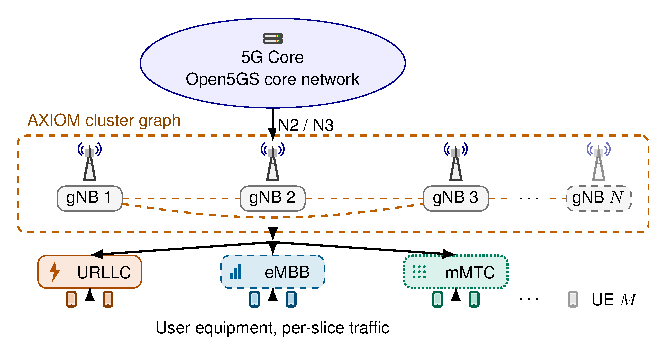
\includegraphics{Fig1}
\caption{Conceptual system view. A cluster of $N$ gNBs, coordinated by the shared
AXIOM encoder and backhauled to a 5G core, serves $M$ user equipment (UE) devices across three slices.
AXIOM is evaluated offline, and the live rig runs one gNB}
\label{fig:sysview}
\end{figure}

This paper introduces AXIOM, an acronym for Adaptive Cross-cell Integrated Orchestration of Multi-slice admission. It is designed for the Open Radio Access Network (O-RAN), a softwarised RAN architecture with open, standardised interfaces between its components. One encoder, shared by every gNB, feeds a separate Q-head for each slice, under centralised training and decentralised execution. The encoder is a graph attention network (GAT)~\cite{wu2021gnnsurvey}, and the per-slice heads, each a small multi-layer perceptron (MLP), carry AXIOM's advantage as the cluster grows. Attention itself adds nothing measurable, as Section~\ref{sec:results-ablation} shows. Three gaps found in our prior systematic review of 67 core studies motivate pairing AXIOM with a stricter evaluation, as Section~\ref{sec:litreview} details. No reviewed study checks whether its outcome metric can score a degenerate policy, such as one that accepts every request, as well as a correct one, which blocks just enough low-priority requests to protect the priority slices. In addition, none replicates a headline finding on an independent seed sample, and none tests whether a live testbed reaches the contention that its offline claims assume. A seed fixes the random draws of one run, such as its starting weights and the traffic it trains and is tested on. A finding that also holds on seeds never used before is therefore unlikely to be an artefact of one sample.

We evaluate AXIOM in two offline simulators of a gNB cluster. Firstly, we consider a simple environment (Env A) with a static load, where shedding every mMTC request is close to optimal. Secondly, we consider Env B, which adds time-varying load and inter-cell coupling, so shedding one fixed slice is no longer optimal. We then compare AXIOM with a single-agent deep Q-network (DQN-SA), independent per-gNB deep Q-networks (DQN-I), multi-agent proximal policy optimisation (MAPPO), and tuned threshold rules. We also grow the cluster to 7, 19, and 37 gNBs under three layouts. Further campaigns test federated averaging (FedAvg), differential privacy, and network disruption. The contributions of this paper are as follows.
\begin{enumerate}
\item AXIOM, a slice-admission controller with a shared cluster encoder and decentralised per-slice Q-heads, whose parameter count does not grow with the cluster and whose per-slice heads, rather than attention, carry its advantage at scale. A policy trained at seven gNBs runs unchanged at 19 and 37 gNBs and keeps above 95\% priority-slice compliance there in Env A.
\item Env A, a shared-budget environment with static load, built after a trivial-policy check showed that accepting every request beat every learned policy in our original simulator. In Env A, AXIOM keeps priority-slice compliance above 93\% at 7, 19, and 37 gNBs, while both DQN baselines and MAPPO stay below 84\%.
\item Env B, a more demanding environment with time-varying load and inter-cell coupling. There AXIOM leads DQN-SA, DQN-I, and MAPPO at three and nineteen gNBs and beats a static shedding rule at three, while a tuned threshold rule sets a bar that no learned policy reaches under its tuning conditions.
\item An evaluation protocol for learned slice admission control that combines trivial-policy checks, per-slice correctness metrics, independent-seed replication, tuned rule baselines, and a pre-registered analysis. It applies established practice for evaluating reinforcement learning~\cite{henderson2018matters,agarwal2021precipice} to slice admission and adds trivial-policy checks that this domain needs.
\end{enumerate}

The remainder of this paper is organised as follows. Section~\ref{sec:litreview} reviews related work, Section~\ref{sec:system-model} formulates the admission problem, and Section~\ref{sec:methodology} presents the AXIOM architecture. Section~\ref{sec:setup} describes the experimental setup and evaluation safeguards, and Section~\ref{sec:results} reports the results. Finally, Section~\ref{sec:discussion} discusses the limitations, and Section~\ref{sec:conclusion} concludes the paper.

\section{Related Work}
\label{sec:litreview}
Our prior systematic review~\cite{ref:access} screened 6{,}286 records down to 67 core studies from 2024 to 2026 on machine-learning-driven, user-centric distributed network slicing. The review organised them around three enabling pillars, namely topology-aware graph representation, distributed multi-agent control, and privacy-preserving federation. Each pillar is well developed on its own, but they are rarely combined under realistic constraints, and never jointly validated in a live deployment.

Studies from the review's core sample show the state of each pillar. Learned admission control uses sequential twin actor-critics~\cite{ojijo2024sac} and digital-twin-accelerated deep reinforcement learning~\cite{tao2025dtac}. Multi-agent control spans sample-efficient multi-agent DQNs for inter-slice orchestration~\cite{doanis2024madqn}, scalable frameworks for dynamic RAN slicing~\cite{li2026scalablemarl}, and cooperative agents for energy-efficient slicing~\cite{phyu2025icecream}. A graph neural network with meta-learning makes bandwidth allocation scalable and transferable~\cite{hao2024hybridtask}, and Ahmadi et al.~\cite{ahmadi2024generalizable} study topology generalisation through attention. Federated deep reinforcement learning has been applied to splitting virtual network functions~\cite{amiri2024vnf} and to slice mobility~\cite{ming2024fedslice}. Two core studies combine two of the three pillars, graph attention with multi-agent learning for task offloading~\cite{mohajer2026pronto} and a graph neural network with multi-agent learning for resource orchestration~\cite{bouroudi2025gnnmarl}. Closest to our evaluation concern, Tsampazi et al.~\cite{tsampazi2025pandora} compare many deep reinforcement learning agents for O-RAN in an automated pipeline, a comparison that our trivial-policy and independent-seed checks extend. None of these core studies checks its metric against a trivial policy or replicates a finding on independent seeds.

\begin{table}[!htbp]
\caption{Closest prior work}
\label{tab:related}
\centering
\footnotesize
{\setlength{\tabcolsep}{2pt}
\begin{tabular}{@{}>{\raggedright\arraybackslash}p{2.45cm}>{\raggedright\arraybackslash}p{3.6cm}ccccccc@{}}
\toprule
Work & Problem & \begin{tabular}[b]{@{}c@{}}Multi-\\agent\end{tabular} & \begin{tabular}[b]{@{}c@{}}Graph\\encoder\end{tabular} & \begin{tabular}[b]{@{}c@{}}Feder-\\ated\end{tabular} & \begin{tabular}[b]{@{}c@{}}Max\\cells\end{tabular} & \begin{tabular}[b]{@{}c@{}}Size-\\invariant\\params\end{tabular} & \begin{tabular}[b]{@{}c@{}}Zero-shot\\size\\transfer\end{tabular} & \begin{tabular}[b]{@{}c@{}}Rule\\base-\\lines\end{tabular} \\
\midrule
Shao et al.~\cite{shao2021gatmarl} & Slicing resource management in dense cells & \gyes & \gyes$^{a}$ & \gnr & 19 & \gnr & \gnr & \gyes \\
Sulaiman et al.~\cite{sulaiman2023coordinated} & Joint slicing and slice admission in cloud RAN & \gyes & \gnr & \gnr & \gnr & \gnr & \gnr & \gyes \\
Ahmadi et al.~\cite{ahmadi2024generalizable} & RAN and edge-computing slicing with admission control & \gyes & \gyes$^{a}$ & \gnr & \gnr & \gnr & \gnr & \gnr \\
Zangooei et al.~\cite{zangooei2024flexible} & SLA-constrained RAN slicing in O-RAN & \gyes & \gnr & \gnr & 1 & \gpart$^{e}$ & \gpart$^{e}$ & \gno \\
Mohajer et al.~\cite{mohajer2026pronto} & SLA-aware task offloading and service orchestration & \gyes & \gyes$^{a}$ & \gnr & \gnr & \gnr & \gnr & \gnr \\
Bouroudi et al.~\cite{bouroudi2025gnnmarl} & Energy-efficient network-function placement & \gyes & \gyes$^{b}$ & \gnr & \gnr & \gnr & \gnr & \gnr \\
\midrule
AXIOM & Per-slice admission across a gNB cluster & \gyes & \gyes$^{c}$ & \gyes$^{d}$ & 37 & \gyes & \gyes & \gyes \\
\botrule
\end{tabular}}
\par\smallskip
{\raggedright\scriptsize \gyes{} reported, \gpart{} partly, \gno{} not used, \gnr{} not reported in the work. $^{a}$Attention. $^{b}$Graph neural network. $^{c}$Shared GAT or MLP. $^{d}$FedAvg variant. $^{e}$Over the number of slices in a single cell, not over cells.\par}
\end{table}

Apart from the core studies above, the works cited in the rest of this section lie outside the review's 67 core studies. They add earlier foundations, studies published in this journal, and further recent work. AXIOM also sits inside the broader O-RAN effort to run learned control loops over standard interfaces, which Polese et al.~\cite{polese2023oran} survey and which ColO-RAN~\cite{polese2023coloran} and Tsampazi et al.~\cite{tsampazi2023xapps} exercise on large experimental platforms. Learned slice admission predates O-RAN, from market-driven admission~\cite{bega2020market} to reinforcement learning for RAN slicing~\cite{raza2019slicing}, and Khani et al.~\cite{khani2024sacsurvey} survey it for cloud RAN. OACR$^{2}$~\cite{li2025oacr2} uses request forecasting to maximise the infrastructure provider's long-term revenue. AXIOM instead protects priority-slice SLAs, the objective of an operator bound by strict per-slice guarantees. Cooperative agents usually train by value factorisation such as QMIX~\cite{rashid2020qmix} or with a centralised critic as in MAPPO~\cite{yu2022mappo}, and constrained multi-agent learning has been applied to O-RAN slicing at scale~\cite{zangooei2024flexible}. Recent work in this journal applies actor-critic learning~\cite{kulkarni2024actor} and double deep Q-networks~\cite{kamal2026ddqn} to related problems. Other studies in it address delay-aware allocation~\cite{alqahtani2025dynamic}, federated learning~\cite{krishnamoorthy2026federated}, and multi-agent relay selection~\cite{sirma2025relay}. None of these studies checks its metric against a trivial policy or replicates on independent seeds. Such checks have overturned published results in other areas of networking. In optical networks, Doherty et al.~\cite{doherty2025hype} recreated five landmark reinforcement learning studies of resource allocation and found that simple tuned heuristics outperformed the published learned allocators. Our trivial-policy and tuned-rule checks bring the same scrutiny to slice admission. For slice admission itself, Asdikian et al.~\cite{asdikian2025verifying} attribute a learned agent's decisions to its input features with Shapley values, so that operators can verify its behaviour before deployment. Our checks on the metric complement this view of the policy. Unlike the learned controllers above, AXIOM shares one encoder across agents and gives every slice its own decision head, which Section~\ref{sec:results-ablation} shows matters as the cluster grows.

Two further works come close on a single axis of this problem. Shao et al.~\cite{shao2021gatmarl} show that graph attention strengthens inter-agent cooperation. Sulaiman et al.~\cite{sulaiman2023coordinated} are the closest prior art to joint slicing and admission control, yet neither study checks for degenerate policies or replicates on independent seeds. Table~\ref{tab:related} sets AXIOM beside the six closest works from both groups, and none of them pairs per-slice admission with a size-independent shared controller and evaluates it against trivial and tuned rules on independent seeds.

Robustness studies~\cite{tashman2026adversarial,fatehi2026attentionmarl} test disruptive conditions, as our disruption campaign does, yet neither checks whether its robustness metric is trustworthy or replicates a finding. Zhang et al.~\cite{zhang2022federatedoran} and Yasin et al.~\cite{yasin2025dpfl} are the closest precedents for periodic synchronisation and for federated learning with differential privacy, but both secure the controller rather than characterise a control policy's own privacy-utility trade-off. Gong et al.~\cite{gong2026femaddpg} combine federated training with multi-agent control, two of the three pillars. Like every work above, each of these evaluates its own outcome metric once, on one seed or run.

\section{System Model and Problem Formulation}
\label{sec:system-model}
This section formulates slice admission across a gNB cluster as a decentralised decision problem and describes the two simulators that evaluate it. We consider a cluster of $N$ gNBs, from three in the main campaigns to 37 in the scaling study. Each gNB serves URLLC, eMBB, and mMTC under a shared per-gNB Physical Resource Block (PRB) budget $B$. At each control step every gNB holds zero or more pending requests, each tagged with a slice, and its agent accepts or rejects each one, conditioned on the cluster state. Each decision moves the slice's PRB-ratio ceiling, the control that OpenAirInterface (OAI) exposes to xApps, the external control applications of O-RAN. The binary action matches our single-gNB work, so any coordination benefit comes from the architecture. At three gNBs the cluster is treated as fully connected, a modelling choice, and the scaling study adds ring and hex-grid layouts. The model works at the PRB level and abstracts the radio channel. Channel quality changes how many PRBs a slice needs for the same traffic, and the model folds this into the per-step demand noise. A channel-aware extension that maps the signal-to-interference-plus-noise ratio to PRB demand is left to future work.

The step reward follows our earlier formulations~\cite{mecon-paper1,icraie-paper2}. It combines a per-slice service term net of SLA-violation penalties with a congestion charge on admitted volume and a load-imbalance penalty. For slice $k$, $\omega_k$ is the priority weight and $R_k$ the per-accept reward. Its admitted count is $n_k$ and its violation penalty $\lambda_k$, and $\mathbf{1}[v_k]$ flags an SLA violation in that step. With these terms, the reward of step $t$ is then
\begin{equation}
\label{eq:reward}
r_t = \sum_{k}\!\big(\omega_k R_k\, n_k - \lambda_k\,\mathbf{1}[v_k]\big)
      \;-\; \kappa\, C_t \lVert \mathbf{a}_t \rVert_1
      \;-\; \beta\,(1 - F_t),
\end{equation}
where $\lVert \mathbf{a}_t \rVert_1$ is the total admitted this step and $C_t$ the cluster-mean congestion level. The congestion coefficient is $\kappa$, and $F_t\!\in\![0,1]$ is the min-over-max PRB-utilisation fairness ratio with load-balance weight $\beta$. The violation flag $v_k$ follows from a continuous SLA margin $m_k$. The correctness-aware metrics of Section~\ref{sec:collapse} also build on this margin. We take it as the worse of the queue and loss channels,
\begin{equation}
\label{eq:margin}
m_k = \min\!\Big(1 - \tilde q_k,\; 1 - \tfrac{\ell_k}{\ell_k^{\max}}\Big),
\qquad v_k \Leftrightarrow m_k \le 0,
\end{equation}
with $\tilde q_k$ the slice backlog relative to its budget, and $\ell_k$ and $\ell_k^{\max}$ its loss proxy and loss budget. The weights rank the slices by the cost of a missed SLA. URLLC carries time-critical traffic with the tightest budgets, 15 ms of latency and 0.8\% loss, so it has the largest weight and penalty and is never the slice to shed. eMBB carries throughput-heavy traffic with looser budgets, and mMTC carries small, delay-tolerant device reports with the loosest budgets and the smallest weight. Under congestion the intended policy is therefore differentiated shedding, which sheds mMTC first, sheds eMBB only when URLLC's queue builds, and keeps accepting URLLC.

Admission is therefore a decentralised partially observable Markov decision process. At step $t$ the state $s_t$ comprises every gNB's queues, offered demand, and slice ceilings. Agent $i$ observes its own feature row $\mathbf{x}_i$, which the shared encoder combines with the other rows of $\mathbf{X}_t$. For each pending request it chooses $a\in\{\text{accept},\text{reject}\}$, the shared-budget dynamics move the cluster to $s_{t+1}$, and every agent receives the common reward $r_t$ of Eq.~\eqref{eq:reward}. The agents jointly seek a policy $\pi$ that maximises the discounted return over an episode of $T{=}60$ steps,
\begin{equation}
\max_{\pi}\;\mathbb{E}_{\pi}\Big[\textstyle\sum_{t=0}^{T-1}\gamma^{t} r_t\Big],\qquad \gamma=0.95.
\end{equation}

\begin{table}[!t]
\caption{Simulation and training parameters not stated in the text, shared by both environments}
\label{tab:params}
\centering
\footnotesize
{\setlength{\tabcolsep}{3pt}
\begin{tabular}{@{}>{\raggedright\arraybackslash}p{96pt}*{3}{>{\centering\arraybackslash}p{86pt}}@{}}
\toprule
Slice parameter & URLLC & eMBB & mMTC \\
\midrule
Floor and cap, PRB ratio & 5 to 33 & 10 to 66 & 5 to 11 \\
Priority weight $\omega_k$ & 12.0 & 3.5 & 0.3 \\
Violation penalty $\lambda_k$ & 10.0 & 5.0 & 2.5 \\
Per-accept reward $R_k$ & 1.0 & 1.0 & 1.0 \\
Latency budget (ms) & 15 & 45 & 65 \\
Loss budget (\%) & 0.8 & 2.0 & 3.5 \\
\midrule
\multicolumn{4}{@{}l}{Simulator} \\
\cmidrule(r){1-4}
Congestion $\kappa$, balance $\beta$ & \multicolumn{3}{>{\raggedright\arraybackslash}p{270pt}@{}}{1.5, 1.0} \\
Episode & \multicolumn{3}{>{\raggedright\arraybackslash}p{270pt}@{}}{60 steps of 5 s, queues emptied at start} \\
Requests per step & \multicolumn{3}{>{\raggedright\arraybackslash}p{270pt}@{}}{$N$, uniform slice and gNB, at most $4N$ pending} \\
Demand noise, gate step & \multicolumn{3}{>{\raggedright\arraybackslash}p{270pt}@{}}{$0.005B$ per step, 5 PRB-ratio points per decision} \\
\midrule
\multicolumn{4}{@{}l}{Learning} \\
\cmidrule(r){1-4}
Value-based learners & \multicolumn{3}{>{\raggedright\arraybackslash}p{270pt}@{}}{Adam, learning rate $10^{-3}$, $\epsilon$ from 1.0 to 0.05 at $\times0.985$ per episode, replay 10,000, minibatch 16, warm-up 32, target sync every 10 episodes} \\
AXIOM network & \multicolumn{3}{>{\raggedright\arraybackslash}p{270pt}@{}}{Two-layer, four-head GAT, hidden and output 16, raw-feature skip, per-slice Q-heads of hidden 32, Huber loss, gradient clip 1.0} \\
DQN baselines & \multicolumn{3}{>{\raggedright\arraybackslash}p{270pt}@{}}{Two hidden layers of 128, squared-error loss} \\
MAPPO & \multicolumn{3}{>{\raggedright\arraybackslash}p{270pt}@{}}{Learning rate $10^{-3}$, 10 epochs, minibatch 64, clip 0.2, entropy 0.01, advantage $\lambda=0.95$} \\
\botrule
\end{tabular}}
\end{table}

Each gNB has a budget of $B{=}100$ PRBs in both simulators. The nominal shares are 30, 60, and 10 PRBs for URLLC, eMBB, and mMTC. Each slice's mean offered demand is 105\% of its share, scaled by a fixed per-gNB multiplier $m_i$ between 0.9 and 1.0. This puts a gNB's mean demand at about 95\% to 105\% of its budget, before per-step noise and backlog. When admitted demand exceeds $B$, the slices share it in proportion to demand, so every admitted mMTC request takes resources from URLLC and eMBB. Unserved demand carries forward as backlog within an episode. Each episode starts with empty queues and every slice ceiling at its nominal share. An accept raises a slice's ceiling by 5 PRB-ratio points, up to its cap, and a reject lowers it by 5 points, down to its floor, and relieves one request's demand from the backlog. Each slice then asks for the smaller of its offered demand plus backlog and its ceiling, and the offered PRBs drift 10\% per step towards their mean, with noise of $0.005B$. Env B keeps all of this and adds two mechanisms. Each gNB's mean demand follows $0.95\,(1+0.3\sin(2\pi(s+\psi_i)/60))$ times its nominal shares, again scaled by $m_i$, with $s$ the step and $\psi_i$ a phase redrawn per gNB and episode. As a result, demand swings between about 60\% and 124\% of the budget. A gNB's usable budget also shrinks with its neighbours' previous load, $B_i(t)=B\,(1-0.15\,\bar u_{\mathcal{N}(i)}(t-1))$, a first-order model of inter-cell interference over the same adjacency graph the encoder reads. In Env B shedding every mMTC request leaves URLLC compliance at 62.5\% at three gNBs, whereas a rule that also sheds eMBB when the URLLC queue builds keeps it at 98.9\%. Per-slice compliance counts a slice as compliant only when every gNB meets it, which saturates in Env B at nineteen gNBs, so there we also report per-gNB compliance. Fig.~\ref{fig:envflow} traces one control step of both simulators, and Table~\ref{tab:params} lists the remaining simulation and training parameters.

\begin{figure}[!htbp]
\centering
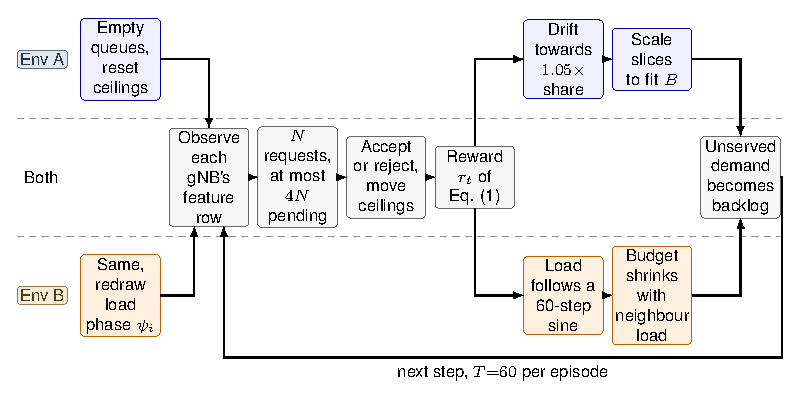
\includegraphics[width=119mm]{Fig2}
\caption{One control step of both simulators, repeated for $T{=}60$ steps per episode. The middle lane holds the steps both share, and the outer lanes the steps where Env A and Env B differ. The text gives each step in full}
\label{fig:envflow}
\end{figure}

\section{The AXIOM Architecture}
\label{sec:methodology}
This section presents the AXIOM architecture, its training rule, and its federated variant. AXIOM differs from its DQN baselines in what each policy sees and shares. AXIOM trains one encoder over the whole cluster from every agent's experience and reads out one Q-head per slice. DQN-SA is one controller over a flattened joint state, and DQN-I gives each gNB its own learner over local features only. The two baselines are therefore ablations that remove the shared encoder.

\begin{figure}[!htbp]
\centering
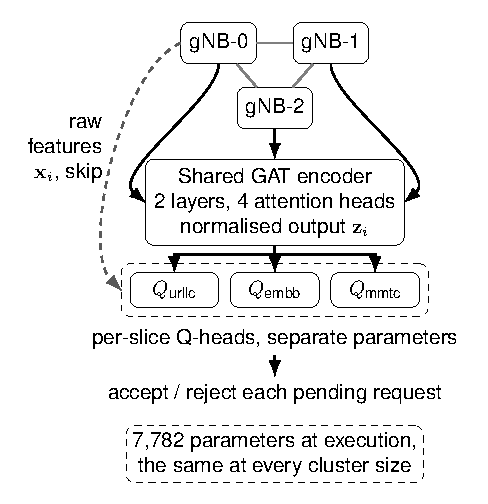
\includegraphics[width=119mm]{Fig3}
\caption{AXIOM architecture. A shared graph-attention encoder produces one embedding per gNB, and per-slice Q-heads read that gNB's embedding and raw features. Training on every agent's requests is centralised, and each gNB acts on its own row}
\label{fig:architecture}
\end{figure}

\begin{algorithm}[!htbp]
\caption{Centralised training and decentralised execution of AXIOM}
\label{alg:gat-ctde}
\begin{algorithmic}[1]
\REQUIRE encoder $f_\theta$, per-slice Q-heads $\{Q_{\phi_k}\}$, targets $f_{\theta^-},\{Q_{\phi_k^-}\}$, buffer $\mathcal{D}$, adjacency $\mathbf{A}$, discount $\gamma$, sync period $T_{\mathrm{s}}$
\FOR{each step $t$, observing joint node features $\mathbf{X}_t$}
  \STATE $\mathbf{E}_t \gets f_\theta(\mathbf{X}_t, \mathbf{A})$ \COMMENT{centralised, one row per gNB}
  \FORALL{pending requests at gNB $i$, slice $k$}
    \STATE $a \gets \arg\max_a Q_{\phi_k}([\mathbf{E}_t[i], \mathbf{X}_t[i]])[a]$, $\epsilon$-greedy \COMMENT{decentralised, own row only}
  \ENDFOR
  \STATE step env, store $(\mathbf{X}_t, \mathbf{X}_{t+1}, \{(i,k,a)\}, r_t, \eta_t)$ in $\mathcal{D}$
  \IF{$|\mathcal{D}| \geq$ warm-up}
    \STATE sample minibatch $\mathcal{M}$, then $\mathbf{E}_{\mathcal{M}} \gets f_\theta(\mathbf{X}_{\mathcal{M}},\mathbf{A})$, $\mathbf{E}'_{\mathcal{M}} \gets f_{\theta^-}(\mathbf{X}'_{\mathcal{M}},\mathbf{A})$
    \STATE per request, $y \gets r + \gamma(1{-}\eta)\max_{a'} Q_{\phi_k^-}([\mathbf{E}'_{\mathcal{M}}[i], \mathbf{X}'_{\mathcal{M}}[i]])[a']$
    \STATE $\mathcal{L} \gets$ mean per-request Huber loss, never summed per step, then update $\theta,\{\phi_k\}$ with gradient norm clipped at 1.0
  \ENDIF
  \STATE every $T_{\mathrm{s}}$ episodes, $\theta^-\gets\theta$, $\phi_k^-\gets\phi_k$
\ENDFOR
\end{algorithmic}
\end{algorithm}

\subsection{Shared Encoder, Decentralised Q-Heads}
\label{sec:methodology-perslice}
Fig.~\ref{fig:architecture} shows the AXIOM architecture and its data flow. At every step each gNB forms a feature row $\mathbf{x}_i$ of its PRB-used ratio, congestion level, and normalised queue length, and the rows stack into $\mathbf{X}\in\mathbb{R}^{N\times d}$. A two-layer, four-head GAT over the adjacency graph maps $\mathbf{X}$ to one normalised embedding $\mathbf{z}_i$ per gNB, and Section S4 of Online Resource 1 gives its attention equations. Every agent's loss updates this encoder, which is centralised training, while each agent decides its own pending requests from its own row $\mathbf{z}_i$, which is decentralised execution.

Two design choices in AXIOM matter most at scale. One small MLP per slice gives each slice its own parameters, so URLLC's large priority weight cannot swamp mMTC's smaller learning signal in a shared head, which Section~\ref{sec:results-ablation} confirms at nineteen gNBs. Each node's raw features are also concatenated onto its normalised embedding before the heads, $Q_{\phi_k}([\mathbf{z}_i,\mathbf{x}_i])$, so a head sees absolute queue and congestion levels. From here on, $\mathbf{z}_i$ denotes that concatenated input to the heads. This skip connection and a learning rate of $10^{-3}$, both chosen on Env B pilot seeds before any reported run, are the only changes from the original AXIOM design.

In training, every pending request at gNB $i$, slice $k$ is its own temporal-difference sample, and Algorithm~\ref{alg:gat-ctde} gives the full training loop. For a request with immediate reward $r$ and next-state embedding $\mathbf{z}_i'$, the target $y$ at discount $\gamma$ and the minibatch loss are
\begin{equation}
y = r + \gamma\,(1-\eta)\max_{a'} Q_{\phi_k^-}\!\big(\mathbf{z}_i'\big)[a'],
\qquad
\mathcal{L} = \frac{1}{|\mathcal{M}|}\sum_{(i,k,a)\in \mathcal{M}}\ell_\delta\!\Big(Q_{\phi_k}(\mathbf{z}_i)[a]-y\Big),
\end{equation}
where $Q_{\phi_k^-}$ is slice $k$'s target Q-head, $\eta\in\{0,1\}$ the flag that marks an episode's last step, $\mathcal{M}$ the minibatch of requests, and $\ell_\delta$ the Huber loss. Section~\ref{sec:results-ablation} shows that a summed per-step target works as well, so the per-request scheme is a simplification rather than a source of AXIOM's advantage.

\subsection{Federated Training with Differential Privacy}
Section S5 of Online Resource 1 shows the federated variant, in which each gNB holds a private copy of the network, trains only on its own requests, and every $N_{\mathrm{loc}}$ local steps sends its weights for FedAvg~\cite{lim2020flmec}. Each client can add differential privacy through a differentially private stochastic gradient descent (DP-SGD) step~\cite{dpsgd}, which clips its minibatch gradient and adds Gaussian noise of multiplier $\sigma$. The privacy loss is accounted for with zero-concentrated differential privacy~\cite{zcdp}. Section S4 of Online Resource 1 gives the clipping, the privacy accounting, and its assumptions.

\section{Experimental Setup}
\label{sec:setup}
This section describes the campaigns, the baselines, and the statistical tests, followed by the safeguards that protect every reported result. The protocol follows established practice for evaluating reinforcement learning~\cite{henderson2018matters,agarwal2021precipice}, with many seeds, interval estimates, and paired tests, and adds trivial-policy checks specific to slice admission. Every campaign uses 300 training and 50 evaluation episodes per seed, where a seed fixes one network initialisation and one environment stream, and each seed is evaluated on a held-out stream. The three-gNB campaigns use 30 seeds, 900 to 929, with a disjoint replication sample, 1000 to 1009. The scaling campaigns use 15 seeds per layout at seven gNBs, 30 at nineteen, and at thirty-seven 30 on the hex layout and 15 on each other layout. MAPPO~\cite{yu2022mappo} is a published multi-agent baseline with a shared actor and a centralised critic, trained on-policy for the same 300 episodes on the same reward. Its learning rate, epochs, and minibatch size were tuned on pilot seeds, because untuned it collapsed in four of five pilot seeds.

\begin{figure}[!htbp]
\centering
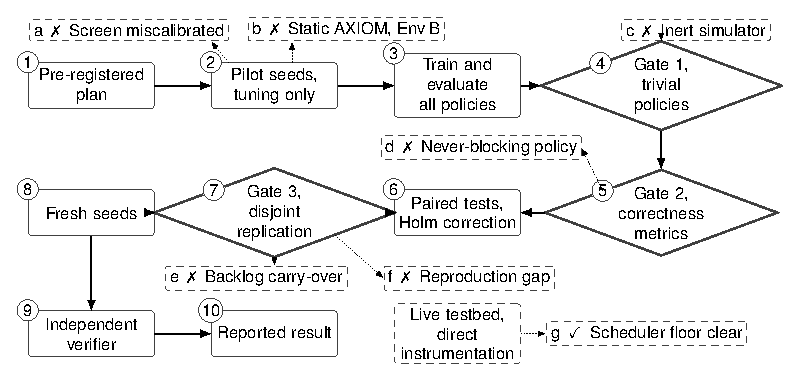
\includegraphics[width=119mm]{Fig4}
\caption{Evaluation protocol in ten steps, with the three gates as diamonds. Dashed callouts name what each check found. a, A miscalibrated validation screen led to an amended plan, back to step 1. b, AXIOM stayed static in Env B, which led to faster learning, back to step 3. c, An inert simulator led to the shared-budget rerun, back to step 3. d, A never-blocking policy is counted as collapsed. e, Backlog carried across episodes led to an episode reset and a rerun, back to step 3. f, A reproduction gap led to a retracted claim. g, The live testbed found no scheduler floor, over more than 100{,}000 readings}
\label{fig:protocol}
\end{figure}

Rules need no learning, and accept-all simply admits every request. A threshold rule sheds mMTC whenever its gNB's congestion level reaches a threshold $\tau$, chosen in Env A on training streams only. Thresholds of 0, 0.5, and 0.8 tie exactly on the training streams, and we keep the lowest, $\tau{=}0$. The rule then sheds every mMTC request, and we call it the static shed-mMTC rule, or static rule for short. Shedding mMTC is the natural first step, since it has the smallest weight and the loosest budgets. In Env A, where demand runs 5\% above the nominal shares, removing it frees enough PRBs to keep URLLC at full compliance and eMBB at 99.98\% on average, as Section~\ref{sec:results-static} shows. It is the best rule of its family on training streams. It is a strong reference rather than a proven optimum, since across our Env A samples learned policies exceeded it in 28 of 450 seed-level evaluations, by at most 0.40 reward per step. In Env B we add two tuned rule families, each chosen on training streams over a grid of thresholds and evaluated on the held-out streams. Operators commonly protect slices with thresholds of this kind, so a learned controller earns its place only by beating the best threshold an engineer could set, and the tuned rules give the learners that bar. The local family sheds mMTC on the gNB's own congestion or priority-slice queue and sheds eMBB on its URLLC queue, while the neighbour-aware family also reads the mean congestion of the gNB's neighbours. eMBB is the second slice to shed. Under Env B's load peaks, shedding mMTC alone cannot protect URLLC, as Section~\ref{sec:results-envb} shows, and eMBB frees the most room, since it has the largest PRB ceiling and the next-smallest weight. Two further runs repeat the DQN baselines at a learning rate of $10^{-4}$.

All learned policies share $\gamma=0.95$, the training budget, and the exploration schedule of Table~\ref{tab:params}, and Section S4 of Online Resource 1 gives the design of the sensitivity studies.

All confidence intervals (CIs) are 95\% bootstrap percentile intervals over 10{,}000 resamples. Paired comparisons use the Wilcoxon signed-rank test, and each family of comparisons against AXIOM is Holm-corrected for multiple testing. The test drops exactly tied pairs, so where two policies make identical decisions on many seeds, as AXIOM and the static rule do in Env A, a comparison rests on the remaining seeds.

The settings, seeds, and four hypotheses of the final campaign were fixed in a pre-registration committed to the project's version-control history before any of its runs, rather than lodged with an external registry. Every later campaign was pre-registered the same way. The Env A baselines that this campaign reuses come from an earlier rerun whose plan was committed one minute after that rerun was launched and before any of its results were read. Section S4 of Online Resource 1 lists the reused results. H1 is that AXIOM beats both trivial rules in Env B, and H2 compares it with every learned baseline and tuned rule in Env B. H3 asks whether graph attention beats a per-node MLP encoder in Env B at seven gNBs, and H4 compares AXIOM with every baseline at nineteen gNBs in Env A.

A pre-registered validation screen checks every trained checkpoint on its own training stream before evaluation. Every seed is reported whether or not it passes, and Section S4 of Online Resource 1 gives the screen's criteria.

\label{sec:collapse}
Three safeguards protect the results, and Fig.~\ref{fig:protocol} places them in the evaluation protocol with the failure each one caught. A trivial-policy check evaluates accept-all and one-slice shedding before any learned policy is trusted, and it exposed an earlier simulator in which accepting every request was optimal.

Correctness-aware metrics form the second safeguard of the evaluation. Block precision $\pi = b_{\text{mMTC}}/b$ is the share of a policy's $b$ blocked requests that target mMTC, and a seed that never blocks counts as a collapse rather than a success. Per-slice SLA compliance then shows whether shedding protects URLLC and eMBB, whereas all-slice compliance scores a correct policy and a failed one alike, because correct shedding gives up mMTC's SLA by design.

Finally, every headline comparison is recomputed on an independent, disjoint seed sample. This caught queue backlog carried over between episodes, and every result here comes from the corrected simulator, which empties all queues at the start of each episode.

\section{Results}
\label{sec:results}
We summarise per-slice compliance as priority-slice compliance, the mean of URLLC and eMBB compliance, and call a trained policy collapsed when it accepts every request. Fig.~\ref{fig:m6-topology} sets out how the four learned policies stand as the cluster grows. Throughout, a reward margin is a difference in mean reward per step, a compliance margin is in percentage points, and a load level is a percentage of the nominal offered demand.

\subsection{Static Load, Three gNBs}
\label{sec:results-static}
In the thirty-seed campaign of Table~\ref{tab:m2-results}, AXIOM never collapses and comes closer to the static rule's reward than any other learner. AXIOM earns 1.110 more reward per step than DQN-I, with 95\% CI [0.60, 1.65]. It earns 2.685 more than MAPPO, with 95\% CI [2.01, 3.35], and both margins hold at Holm-adjusted $p\leq0.0002$. Its margin over DQN-SA, 0.311 with 95\% CI [$-$0.01, 0.64], does not survive correction on thirty seeds, at $p=0.066$. A disjoint replication on seeds 1000 to 1009 and the pooled 40 seeds favour AXIOM more strongly, as Section S5 of Online Resource 1 reports, but fresh seeds in Section~\ref{sec:results-verify} do not reproduce the lead over DQN-SA.

\begin{table}[!htbp]
\caption{Env A, three gNBs, 30 seeds per policy, 95\% bootstrap CIs. Rules above the line, learned policies below it. W/T/L counts the seeds where AXIOM earns more, the same, or less. Precision averages the seeds that block at all}
\label{tab:m2-results}
\centering
\footnotesize
{\setlength{\tabcolsep}{1.8pt}
\begin{tabular}{@{}lS[table-format=2.3]cS[table-format=3.1]cS[table-format=1.3]cS[table-format=3.1]S[table-format=3.1]S[table-format=2.1]@{}}
\toprule
& & & & & & & \multicolumn{3}{c}{Compliance (\%)} \\
\cmidrule(l){8-10}
Policy & {\begin{tabular}[b]{@{}c@{}}Reward\\per step\end{tabular}} & 95\% CI & {\begin{tabular}[b]{@{}c@{}}Of static\\rule (\%)\end{tabular}} & \begin{tabular}[b]{@{}c@{}}AXIOM W/T/L\\($n=30$)\end{tabular} & {Precision} & Collapsed & {URLLC} & {eMBB} & {mMTC} \\
\midrule
Static rule & 12.835 & [12.77, 12.91] & 100.0 & 2/22/6 & 1.000 & 0/30 & 100.0 & 100.0 & 36.6 \\
\midrule
AXIOM & 12.698 & [12.49, 12.86] & 98.9 & -- & 0.992 & 0/30 & 99.8 & 97.9 & 38.9 \\
DQN-SA & 12.387 & [12.11, 12.63] & 96.5 & 15/8/7 & 0.990 & 0/30 & 99.4 & 94.1 & 43.6 \\
DQN-I & 11.587 & [11.11, 12.02] & 90.3 & 27/0/3 & 0.962 & 0/30 & 99.3 & 86.5 & 40.2 \\
MAPPO & 10.013 & [9.30, 10.73] & 78.0 & 29/1/0 & 0.707 & 2/30 & 97.8 & 57.6 & 66.4 \\
\botrule
\end{tabular}}
\end{table}

\subsection{Cluster-Size Scaling}
We grow the Env A cluster from three gNBs to seven and nineteen under fully-connected, ring, and hex-grid layouts. A pre-registered extension then adds a thirty-seven-gNB cluster on the same layouts. We test the per-layout gaps on reward and on priority-slice compliance, Holm-correcting the 18 comparisons at each size. Fig.~\ref{fig:m6-topology} traces the result across sizes, and Section S6 of Online Resource 1 gives the per-slice detail.

\begin{figure}[!htbp]
\centering
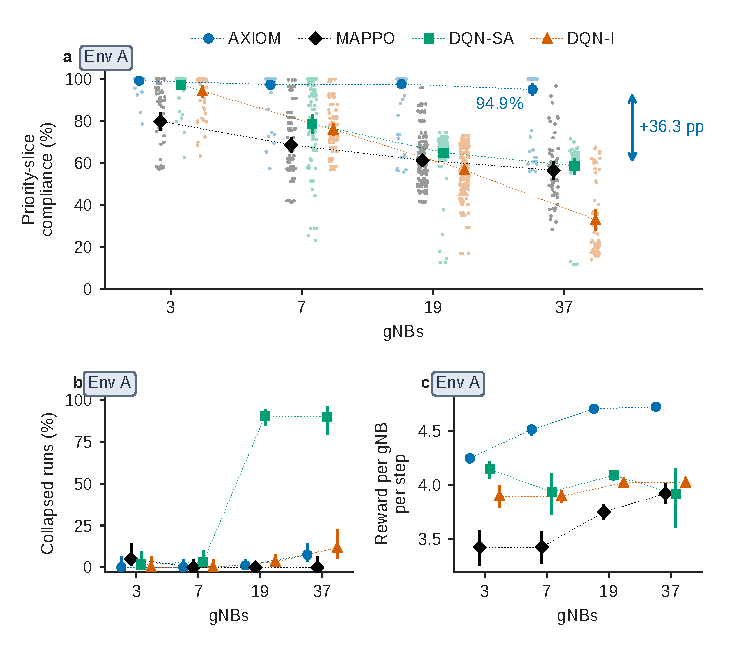
\includegraphics{Fig5}
\caption{Env A as the cluster grows, all layouts pooled, with the layout-independent baselines run once per seed at 37 gNBs. a, Priority-slice compliance, one dot per run, with the mean and 95\% CI. b, Share of trained policies that collapse into accept-all, with Wilson 95\% intervals. c, Reward per gNB per step, mean and 95\% CI. Dotted lines join each policy's means across sizes}
\label{fig:m6-topology}
\end{figure}

At seven gNBs, under every layout, AXIOM keeps 17.9 to 29.9 percentage points more priority-slice compliance than each baseline and earns 3.40 to 7.07 more reward per step. All 18 comparisons hold after Holm correction, at adjusted $p\leq0.011$. At nineteen gNBs the gaps widen, and they answer hypothesis H4. AXIOM keeps a pooled priority-slice compliance of 97.3\% with 95\% CI [95.2\%, 99.0\%]. Under every layout AXIOM keeps 31.0 to 42.1 percentage points more compliance than every baseline and earns 10.7 to 18.6 more reward per step, winning 28 to 30 of 30 seeds. All 18 comparisons hold after Holm correction, at adjusted $p\leq0.0001$.

\begin{figure}[!b]
\centering
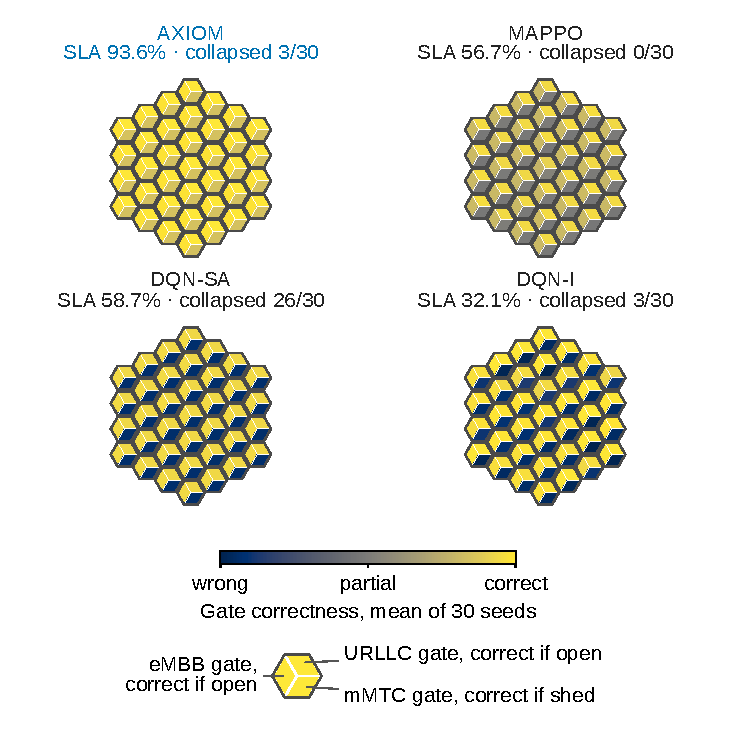
\includegraphics{Fig6}
\caption{Decision map of the 37-gNB hex cluster in Env A over 30 seeds. Each hexagon is a gNB at its true position, split into its URLLC, eMBB, and mMTC admission gates, each drawn on the correctness scale below. Headers give each policy's priority-slice compliance on this layout and its collapsed seeds}
\label{fig:gnb-map}
\end{figure}

At thirty-seven gNBs the lead grows further, and AXIOM keeps a pooled priority-slice compliance of 93.7\% with 95\% CI [89.8\%, 97.2\%]. Under every layout AXIOM keeps 32.0 to 67.8 percentage points more compliance than every baseline and earns 18.3 to 29.5 more reward per step. Here all 18 comparisons hold after Holm correction within their pre-registered families, at adjusted $p<0.01$. AXIOM collapses more often than at nineteen gNBs, as Fig.~\ref{fig:m6-topology}b shows, but even its collapsed runs keep 59\% to 65\%, the level of the best baselines. A pre-registered replication on 20 fresh seeds confirms the result. There AXIOM keeps 95.1\% priority-slice compliance against 34.1\% to 58.5\% for the baselines and leads each on compliance and on reward at Holm-adjusted $p<0.001$. It collapses in 1 of the 20 seeds, against 18 for DQN-SA. On these clusters AXIOM serves 99.8\% of the offered URLLC demand and 99.0\% of the eMBB demand, against 94.2\% to 97.7\% and 85.7\% to 97.5\% for the learned baselines. Its URLLC delay, the mean backlog over the mean served PRBs in 5 s control periods, is 0.08 with a 95th percentile of 0.42, whereas the baselines reach 0.58 to 3.61 with 95th percentiles of 5.2 to 16.9. Section S8 of Online Resource 1 gives throughput and delay in every setting.

Accepting every request is the natural floor at scale. It keeps 70.9\%, 67.1\%, and 61.9\% priority-slice compliance at seven, nineteen, and thirty-seven gNBs. Every baseline falls below it on average at the two larger sizes. AXIOM stays 26 to 32 points above the floor. Its advantage at scale therefore lies in reliably learning the correct shedding policy, the one the static rule encodes, rather than in coordination beyond that rule. The static rule that sheds every mMTC request keeps 99.96\% to 99.99\% at every size. A local threshold rule tuned on Env A training streams at thirty-seven gNBs, in a further pre-registered run, settles on this same policy and matches the static rule in all 30 seeds. Where that rule is known, AXIOM comes within 3 points of it up to nineteen gNBs and within 6.3 at thirty-seven, while from seven gNBs up every other learner falls at least 24 points short. Tuning the DQN baselines on pilot seeds does not close the gap, and AXIOM beats each tuned baseline on compliance and on reward at Holm-adjusted $p<0.001$, by 29.9 to 48.1 points. The published value-decomposition network (VDN)~\cite{sunehag2018vdn} ties AXIOM at three gNBs but trails it by 13.6 points at nineteen, as Section S6 of Online Resource 1 reports.

Fig.~\ref{fig:gnb-map} shows where the gap comes from, gNB by gNB, in the thirty-seven-gNB hex cluster. A gNB's admission gate for a slice is the PRB-ratio ceiling that its accept and reject decisions move between the slice's floor and cap, averaged over every evaluation step of all 30 seeds. AXIOM keeps the URLLC and eMBB gates open at every gNB, at 1.00 and 0.98, and closes the mMTC gate to 0.16 even with its three collapsed seeds included. No baseline closes the mMTC gate below 0.51.

AXIOM's encoder and heads have the same shape at every cluster size, so a policy trained at one size can run unchanged at another. A pre-registered run evaluated the seven-gNB checkpoints, never retrained, at nineteen and thirty-seven gNBs on each seed's held-out stream, and Table~\ref{tab:transfer} gives the result on the 15 seven-gNB seeds. In Env A on the hex layout, AXIOM transferred from seven gNBs keeps 96.2\% and 95.4\% priority-slice compliance at nineteen and thirty-seven gNBs. Accepting every request keeps 65.9\% and 61.1\%, and MAPPO transferred the same way keeps 64.2\% and 61.5\%. All four of AXIOM's leads hold at Holm-adjusted $p=0.00024$. On all three layouts and in Env B at nineteen gNBs, the transferred policy stays within 3.4 points of AXIOM trained at the target size, and no paired difference is significant, with $p\geq0.068$. On 20 fresh seeds trained for this check, AXIOM moved from seven gNBs keeps 96.2\% at nineteen gNBs and 95.2\% at thirty-seven. It beats accept-all and MAPPO moved the same way by 27.0 to 33.8 points, at Holm-adjusted $p<0.001$. The DQN baselines cannot transfer, since DQN-SA reads the joint state of every gNB and DQN-I holds one network for each gNB, with none for the new ones. The Env A result partly reflects how simple the task is there, because the transferred policy earns exactly the size-independent static rule's reward on 9 to 11 of 15 seeds and less on the rest.

\begin{table}[!htbp]
\caption{Zero-shot transfer on the 15 seven-gNB seeds, priority-slice compliance with 95\% CIs. Policies from 7 were trained at seven gNBs and run unchanged, and AXIOM at $N$ was trained at the target size. Env B gives per-gNB compliance}
\label{tab:transfer}
\centering
\footnotesize
{\setlength{\tabcolsep}{2.2pt}
\begin{tabular}{@{}lS[table-format=2.2]cS[table-format=2.2]cS[table-format=2.1]cS[table-format=2.2]S[table-format=2.1]@{}}
\toprule
& \multicolumn{6}{c}{Priority-slice compliance (\%)} & \multicolumn{2}{c}{Rules (\%)} \\
\cmidrule(lr){2-7}\cmidrule(l){8-9}
& \multicolumn{2}{c}{AXIOM from 7} & \multicolumn{2}{c}{AXIOM at $N$} & \multicolumn{2}{c}{MAPPO from 7} & & \\
\cmidrule(lr){2-3}\cmidrule(lr){4-5}\cmidrule(lr){6-7}
Env, layout, $N$ & {Mean} & 95\% CI & {Mean} & 95\% CI & {Mean} & 95\% CI & {Static} & {Accept all} \\
\midrule
A, hex, 19 & 96.2 & [91.6, 99.9] & 94.6 & [86.9, 100.0] & 64.2 & [56.6, 72.2] & 99.96 & 65.9 \\
A, hex, 37 & 95.4 & [89.6, 99.9] & 94.8 & [87.3, 100.0] & 61.5 & [53.7, 70.2] & 99.99 & 61.1 \\
A, ring, 19 & 96.9 & [91.3, 99.9] & 96.8 & [92.3, 99.9] & 64.2 & [56.8, 72.4] & 99.96 & 65.9 \\
A, ring, 37 & 96.3 & [90.3, 99.7] & 93.2 & [85.3, 100.0] & 61.5 & [53.6, 70.2] & 99.99 & 61.1 \\
A, fully connected, 19 & 96.6 & [90.6, 100.0] & 99.96 & [99.9, 100.0] & 64.2 & [56.8, 72.3] & 99.96 & 65.9 \\
A, fully connected, 37 & 96.3 & [90.1, 100.0] & 94.4 & [85.9, 100.0] & 61.5 & [53.8, 70.0] & 99.99 & 61.1 \\
B, hex, 19 & 79.1 & [76.6, 80.8] & 77.3 & [74.2, 79.8] & 72.9 & [70.1, 75.6] & 79.9 & 66.4 \\
\botrule
\end{tabular}}
\end{table}

\subsection{Ablations and Sensitivity}
\label{sec:results-ablation}
Five checks test where AXIOM's behaviour comes from, as Sections S5 and S7 of Online Resource 1 detail. First, the per-slice Q-heads matter as the cluster grows. A variant with one shared head of matched size ties AXIOM at three gNBs. At nineteen gNBs on the ring layout, however, it collapses in 9 of 15 seeds and keeps only 65.9\% priority-slice compliance against AXIOM's 96.8\% on the same seeds, losing every seed at Holm-adjusted $p<0.001$. Second, graph attention adds nothing measurable to AXIOM. A per-node MLP encoder ties AXIOM in Env A. In Env B at seven gNBs it keeps 1.12 and 0.95 more reward per step on the ring and hex layouts and wins 10 of 15 seeds in each. These leads in the pre-registered test H3 miss significance after Holm correction, at $p=0.061$ and $p=0.095$. On ten fresh ring-layout seeds, however, the MLP encoder led by 1.38 reward per step at $p=0.006$. Third, a variant with one joint summed target in place of per-request samples is never significantly different. Fourth, the learning rate matters, and AXIOM stays within 0.13 of the static rule's reward under changed load and slice weights. A 24-configuration MAPPO grid and a seeded DQN-SA still lose to AXIOM in every setting tested. Finally, depth-3 decision trees reproduce 86\% to 97\% of AXIOM's held-out decisions in Env B and shed eMBB once the URLLC queue passes 0.21 at three gNBs and 0.28 at seven after 900 training episodes, near the tuned rule's 0.2. Run as a rule, the trees tie AXIOM at seven gNBs, trail it by 0.19 reward per step at three, and never reach the tuned rule.

\subsection{Time-Varying Load with Inter-Cell Coupling}
\label{sec:results-envb}

Table~\ref{tab:envb} and Fig.~\ref{fig:envb} report Env B at three gNBs, where shedding one fixed slice no longer suffices. AXIOM earns 2.495 more reward per step than shedding every mMTC request and 4.476 more than accept-all. Both gaps hold at Holm-adjusted $p<0.0001$, as hypothesis H1 predicted. It also leads every learned policy, by 1.038 reward per step over DQN-I, 1.337 over DQN-SA, and 1.863 over MAPPO, and keeps more priority-slice compliance than each, at Holm-adjusted $p<0.0001$. A tuned rule that also sheds eMBB whenever the URLLC queue passes 0.2 beats every learned policy, earning 0.420 more than AXIOM at $p<0.0001$.

\begin{table}[!htbp]
\caption{Env B, three gNBs, 30 seeds per policy, 95\% bootstrap CIs. Rules above the line, learned policies below it. W/T/L counts the seeds where AXIOM does better, the same, or worse}
\label{tab:envb}
\centering
\footnotesize
{\setlength{\tabcolsep}{2.0pt}
\begin{tabular}{@{}>{\raggedright\arraybackslash}p{3.5cm}S[table-format=1.3]cS[table-format=3.1]ccS[table-format=2.1]S[table-format=2.1]S[table-format=2.1]@{}}
\toprule
& & & & \multicolumn{2}{c}{W/T/L ($n=30$)} & \multicolumn{3}{c}{Compliance (\%)} \\
\cmidrule(lr){5-6}\cmidrule(l){7-9}
Policy & {\begin{tabular}[b]{@{}c@{}}Reward\\per step\end{tabular}} & 95\% CI & {\begin{tabular}[b]{@{}c@{}}Of tuned\\rule (\%)\end{tabular}} & Reward & \begin{tabular}[b]{@{}c@{}}Priority\\SLA\end{tabular} & {URLLC} & {eMBB} & {mMTC} \\
\midrule
Accept all & 4.356 & [4.13, 4.60] & 47.1 & 30/0/0 & 30/0/0 & 44.6 & 26.5 & 95.5 \\
Shed all mMTC & 6.337 & [6.00, 6.67] & 68.5 & 30/0/0 & 30/0/0 & 62.5 & 36.7 & 37.1 \\
Tuned local rule & 9.252 & [9.12, 9.40] & 100.0 & 8/0/22 & 6/0/24 & 98.9 & 36.7 & 39.0 \\
Tuned neighbour-aware rule & 9.041 & [8.93, 9.15] & 97.7 & 13/0/17 & 23/0/7 & 98.8 & 28.3 & 90.1 \\
\midrule
AXIOM & 8.832 & [8.64, 9.03] & 95.5 & -- & -- & 95.8 & 34.4 & 40.6 \\
DQN-SA & 7.495 & [7.20, 7.77] & 81.0 & 29/0/1 & 26/0/4 & 86.6 & 28.4 & 41.2 \\
DQN-I & 7.794 & [7.44, 8.13] & 84.2 & 29/0/1 & 27/0/3 & 91.0 & 27.0 & 44.1 \\
MAPPO & 6.968 & [6.47, 7.45] & 75.3 & 29/0/1 & 24/0/6 & 79.7 & 28.9 & 57.9 \\
\botrule
\end{tabular}}
\end{table}

\begin{figure}[!htbp]
\centering
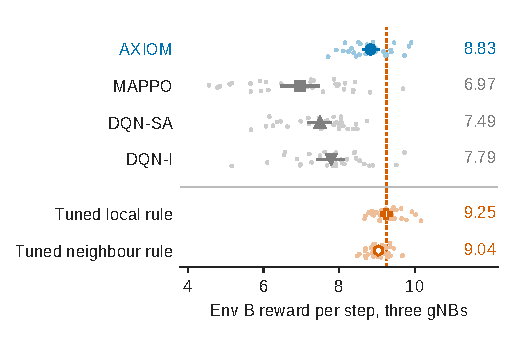
\includegraphics{Fig7}
\caption{Env B reward per step at three gNBs, 30 seeds, with per-seed points behind the mean and 95\% CI. Learned policies are filled markers and rules hollow. The dashed line marks the tuned local rule's mean}
\label{fig:envb}
\end{figure}

At seven gNBs the tuned rules beat AXIOM in all 15 seeds under every layout. On the ring layout AXIOM keeps less compliance than DQN-SA, at Holm-adjusted $p=0.012$. This gap mainly reflects the 300-episode budget, within which 28 of AXIOM's 45 seeds settle on the static rule's policy and never shed eMBB, which none of its 30 seeds does at three gNBs. With 900 episodes for every learner on the ring layout, AXIOM keeps 55.7\% priority-slice compliance against 40.5\% to 42.9\% for the baselines, at Holm-adjusted $p\leq0.0012$, though still below the tuned rule's 60.5\%. After 900 episodes AXIOM rejects eMBB more often as the URLLC queue grows, much as the tuned rule does. At nineteen gNBs the longer budget does not help, and seven of eight seeds keep the static policy after 900 episodes, as Section S7 of Online Resource 1 reports.

At nineteen gNBs, where cluster-level compliance saturates, AXIOM earns 5.54 to 21.22 more reward per step than every learned baseline and keeps 5.5 to 10.9 percentage points more per-gNB priority-slice compliance, at Holm-adjusted $p\leq0.013$. The static rule still earns 1.31 more per step, and the tuned local rule carried over from seven gNBs earns 3.81 more and wins every seed. Fig.~\ref{fig:pergnb} maps this per-gNB compliance for the four learned policies. Each hexagon is one gNB, shaded from dark at 50\% to light at 85\% by the mean share of evaluation steps on which it meets the URLLC and eMBB SLAs. The policies only admit or reject requests where they arrive, so the colours show how well each gNB copes with its own offered load. Every policy keeps the least at the centre gNB, whose load the simulator fixes at the nominal level while it draws every other gNB's from 90\% to 100\% of it. The six inner gNBs have as many neighbours but trail the edge by only 0.5 to 1.8 points. AXIOM keeps more than every learned baseline at each of the nineteen gNBs, by at least 3.8 points, and by at least 4.3 points on the 15 fresh seeds. The carried-over rule leads AXIOM by 13.0 points at the centre and 6.9 points elsewhere, and by 13.2 and 7.0 points on the fresh seeds.

\begin{figure}[!htbp]
\centering
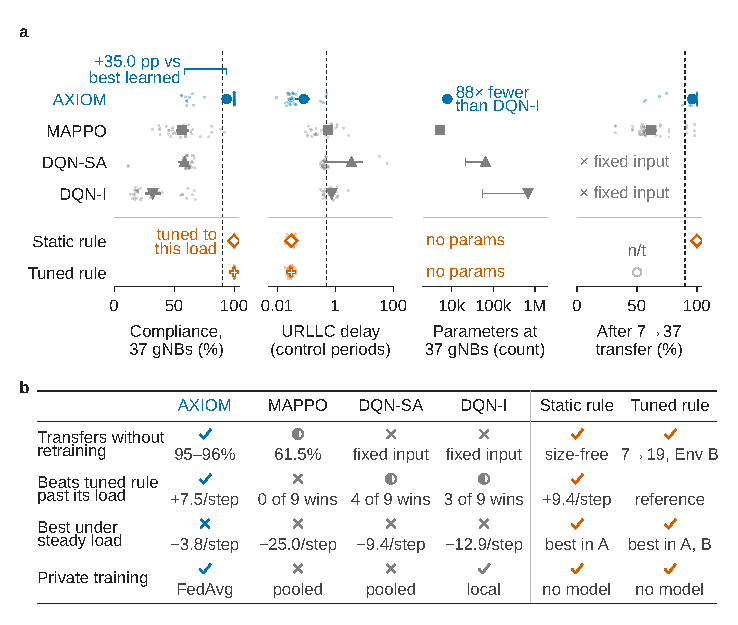
\includegraphics[width=119mm]{Fig8}
\caption{Per-gNB priority-slice compliance in Env B at nineteen gNBs on the hex layout, mean of 15 seeds. a, AXIOM. b, MAPPO. c, DQN-SA. d, DQN-I. The centre gNB is outlined}
\label{fig:pergnb}
\end{figure}

The rule's lead holds only under its tuning conditions. When the load rises to 110\% to 120\% without re-tuning or retraining, AXIOM wins 21 to 23 of 25 seeds at three gNBs, at Holm-adjusted $p\leq0.0002$. At nineteen gNBs it earns 6.23, 7.55, and 8.67 more reward per step than that rule, winning 14 of 15 seeds at each level at Holm-adjusted $p<0.001$. On 15 fresh seeds it leads that rule by 6.84, 8.25, and 9.39 at the same loads, again winning 14 of 15 seeds at Holm-adjusted $p<0.001$, while the rule leads by 3.33 at nominal load. Past the tuning load AXIOM also out-earns MAPPO, DQN-SA, and DQN-I at seven and nineteen gNBs, at Holm-adjusted $p\leq0.008$. At three gNBs it leads all three only at 110\% load, and from 115\% DQN-SA and DQN-I come within 0.21 reward per step of it. A re-tuned rule ties AXIOM up to 115\% load and beats it at 120\%. Section S7 of Online Resource 1 adds uneven per-gNB load and a per-gNB SLA penalty, under which AXIOM still beats every learned baseline but not the rules.

In Env A, Fig.~\ref{fig:m6-topology}a and c show AXIOM staying between 4.2 and 4.7 reward per gNB per step and above 93\% priority-slice compliance, while every baseline loses compliance as the cluster grows. MAPPO is the only learned policy that never collapses at thirty-seven gNBs, where AXIOM collapses in 6 of 60 runs. In Env B every policy loses compliance as the cluster grows, and AXIOM's cluster-level priority-slice compliance falls from 65.1\% at three gNBs to 35.1\% at seven and 24.7\% at nineteen. AXIOM earns the most reward per gNB and keeps the most compliance at three and nineteen gNBs. At seven gNBs it earns 3.36 reward per gNB per step against 3.37 for DQN-SA, which keeps more compliance, 44.3\% against 35.1\%. That gap reflects the training budget, as shown above. In Env A at nineteen gNBs AXIOM stays within 5.3 points of the static rule as offered load rises from 105\% to 120\% of the nominal shares, and every baseline stays below AXIOM at each load.

\begin{table}[!b]
\caption{Design and model complexity at 3, 7, 19, and 37 gNBs. Parameters used at execution, greedy inference time per control step on one CPU thread, and median training time per seed at 3, 19, and 37 gNBs, on the ring layout for AXIOM}
\label{tab:complexity}
\centering
\footnotesize
{\setlength{\tabcolsep}{4pt}
\begin{tabular}{@{}l>{\raggedright\arraybackslash}p{74pt}>{\centering\arraybackslash}p{80pt}cc@{}}
\toprule
Policy & Design & Parameters & ms per step & Training s \\
\midrule
AXIOM & Shared encoder, per-slice heads & 7,782 at every size & 1.04 / 1.98 / 4.79 / 9.89 & 624 / 892 / 1182 \\
DQN-SA & One flattened controller & 21,250 / 26,370 / 41,730 / 64,770 & 0.61 / 1.42 / 3.95 / 8.02 & 85 / 202 / 358 \\
DQN-I & One learner per gNB & 55,302 / 129,038 / 350,246 / 682,058 & 0.59 / 1.38 / 3.73 / 8.08 & 181 / 1054 / 2088 \\
MAPPO & Shared actor, central critic & 5,122 at every size & 0.19 / 0.20 / 0.22 / 0.27 & 73 / 256 / 495 \\
\botrule
\end{tabular}}
\end{table}
\subsection{Model Complexity}

Table~\ref{tab:complexity} sets out the cost of each policy. AXIOM's shared encoder keeps its parameter count fixed as the cluster grows, while the DQN baselines grow with it. Its greedy decisions on one central processing unit (CPU) thread stay well inside the 5 s control period of the live testbed. Against MAPPO, the cheapest learner, the extra cost buys the most where the environment is dynamic. In Env B AXIOM earns 27\% more reward per step than MAPPO at three gNBs and 36\% more at nineteen gNBs. A 24-configuration tuning grid for MAPPO did not close the gap in any setting where it was tested.

\subsection{Reproducibility and Fresh-Seed Verification}
\label{sec:results-verify}
We checked the results in three ways, with every pass criterion fixed before the run it judged. First, rerunning eleven reported settings in fresh processes reproduced every stored result exactly. Sixteen further reruns, from seven to thirty-seven gNBs in both environments, also matched exactly. The one exception is DQN-SA, which builds its network before setting the seed, and seeding it leaves AXIOM's leads unchanged.

Second, four further runs retrained every policy on fresh seeds, 10 to 40 per setting, and 81 of their 90 pre-stated checks held. The nine checks that failed concern secondary margins rather than any headline result. On fresh seeds the DQN baselines reached up to 83.3\% compliance at seven gNBs, above the 80\% bound we had set, and AXIOM's small lead over DQN-SA in Env A at three gNBs did not recur. A fifth fresh-seed run held all three of its checks at thirty-seven gNBs on 20 seeds. A sixth held all four in Env B at nineteen gNBs on 15 seeds, as Section S7 of Online Resource 1 reports. A final pre-registered run held eight of its nine checks. It replicated the transfer and load-shift results on fresh seeds, and the one check that failed, at three gNBs past the tuning load, is reported in Section~\ref{sec:results-envb}. Section S2 of Online Resource 1 compares each reported difference from a learned baseline with its fresh-seed counterpart, and 35 of the 38 whose CI excludes zero hold.

Third, a script written independently of the analysis pipeline, with its own log reader and Holm correction, recomputes the numbers in every results table and the key results sentences from the raw logs. In the current version, all 663 of its checks pass. Section S2 of Online Resource 1 adds interquartile means and probabilities of improvement~\cite{agarwal2021precipice}, and all 51 orderings that this paper draws from means hold under them.

\subsection{Federation, Privacy, Disruption, and Live Deployment}
\label{sec:results-m8}
Federated training costs AXIOM little reward per step on average. Pooled over all 30 federated seeds, ten of them fresh, the cost is $+0.491$ per step with 95\% CI [$-$0.08, 1.09] and $p=0.14$. Even so, a cost of up to about one reward per step cannot be excluded. Per-step DP-SGD noise lowers reward by 0.77 to 1.25 per step without a significant drop, but its formal guarantee is weak, with $\varepsilon$ of about 2{,}600 or more. Under gNB dropout and agent churn every policy loses reward significantly, and no gap between AXIOM and any baseline survives Holm correction at ten seeds. Demand spikes leave AXIOM's decisions largely intact, with block precision at 0.98, and Section S5 of Online Resource 1 gives the protocol. A live single-gNB OAI testbed built on ORANSlice~\cite{cheng2024oranslice} confirmed the control path that AXIOM would use, with 0.000\% loss at one and at two UEs per slice. It never ran short of capacity, however, as Section S3 of Online Resource 1 reports.

\section{Discussion and Limitations}
\label{sec:discussion}
No learned baseline earns significantly more reward than AXIOM in any setting we tested, and its margin over the cheaper MAPPO is largest under time-varying load, coupling, and uneven per-gNB load. A rule known in advance, however, matches or beats AXIOM in steady conditions at every size, and AXIOM beats a tuned rule only when the load moves beyond the rule's tuning conditions. Its practical case is for operators who cannot hand-tune and re-tune rules as conditions change, rather than for a fixed, well-understood cluster. Fig.~\ref{fig:capability} sets out what each controller offers. Among the learned controllers, only AXIOM meets both service thresholds at 37 gNBs and keeps above 90\% compliance when moved there from seven gNBs without retraining. AXIOM learns its own shedding thresholds from the reward, close to those an engineer would tune by hand, and one 7,782-parameter network trained at seven gNBs serves clusters five times larger. The static rule must know in advance which slice to shed, and the tuned rule needs a fresh threshold search whenever conditions change. AXIOM is not retrained after deployment either, so its edge under shifted load comes from what it learned rather than from online adaptation. Fig.~\ref{fig:regime} maps this boundary over every cluster size and load we tested. In Env B AXIOM pulls ahead of the tuned rule at every size from 110\% of the rule's tuning load, and from 105\% at nineteen gNBs. In Env A it never significantly beats the static rule at any size or load. In Env B the static rule also pulls ahead of the tuned rule past its tuning load. At nineteen gNBs it leads the tuned rule by 8.05 to 10.63 reward per step, in all 15 seeds at Holm-adjusted $p<0.001$, and its lead of 1.8 to 2.0 over AXIOM stays within chance, at Holm-adjusted $p\geq0.08$.

\begin{figure}[!htbp]
\centering
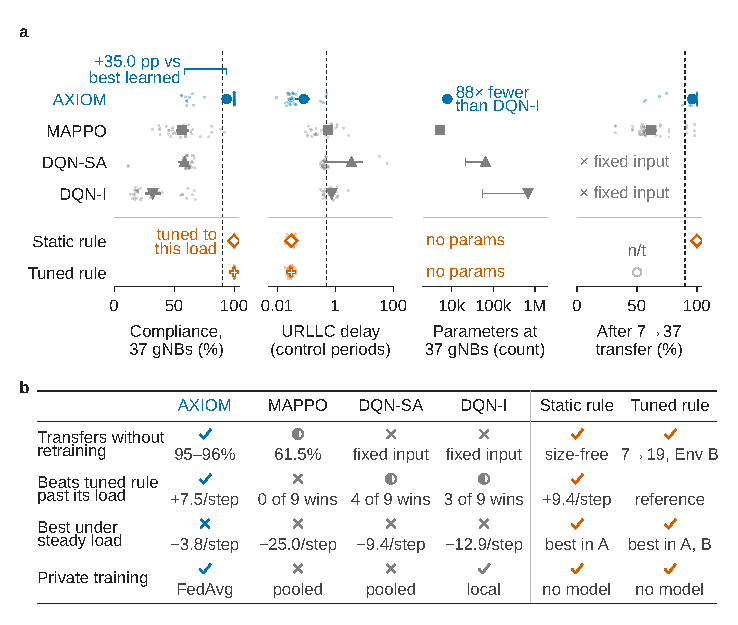
\includegraphics{Fig9}
\caption{What each controller offers. a, Env A at 37 gNBs, with means, 95\% bootstrap CIs, and single seeds as dots. Dashed lines mark 90\% compliance and half a control period of delay, and n/t marks a value not tested. b, Four capabilities, met, partly met, or not met. Reward gaps are per step against the tuned rule in Env B at 19 gNBs. Private training is measured for AXIOM and follows from the training design for the others}
\label{fig:capability}
\end{figure}

\begin{figure}[!htbp]
\centering
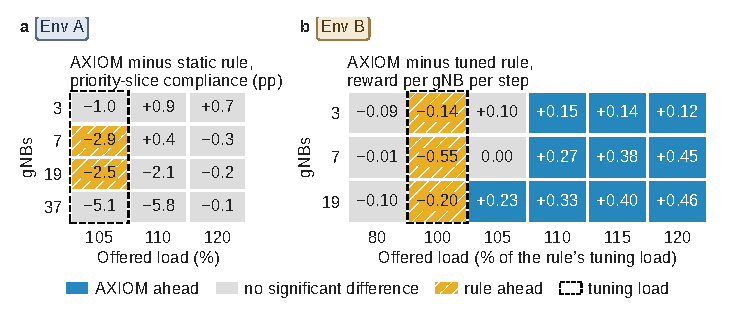
\includegraphics{Fig10}
\caption{Where AXIOM beats or trails a rule tuned once at nominal load, paired per seed. a, Env A priority-slice compliance against the static rule. b, Env B reward per gNB against the tuned rule. Filled cells differ at Holm-adjusted $p<0.05$, hatched where the rule leads. The dashed box marks the rule's tuning load}
\label{fig:regime}
\end{figure}

Several limitations bound the findings of this paper. First, both of our simulators are synthetic rather than measured. They use a first-order coupling model with no radio channel, user mobility, or measured traffic traces, and the live testbed never reached contention. External validity on hardware under load therefore remains the main open question. Future work could drive demand from public cellular activity records, such as the Milan dataset~\cite{barlacchi2015milan}, to test AXIOM under measured load. Second, we did not reimplement a published slice-admission algorithm, so our learned baselines are standard multi-agent methods and ablations of AXIOM rather than prior admission controllers. Third, attention added nothing over a per-node encoder, and a value-decomposition baseline matched AXIOM at three gNBs, so AXIOM's contribution is a design that scales rather than a new learning principle. That per-node variant shares its parameters across gNBs but passes no messages between them, so the gain at scale comes from parameter sharing and per-slice heads. Fourth, the reward charges each slice's SLA penalty once for the cluster, and AXIOM's compliance at seven gNBs depends on that choice. Charging the penalty per violating gNB raised its priority-slice compliance by 10.7 points in Env B at seven gNBs on the ring layout, at Holm-adjusted $p=0.007$. At nineteen gNBs on the hex layout it raised AXIOM's per-gNB compliance by only 1.9 points, at $p=0.65$. Fifth, the load-shift comparison re-tunes rules only offline on shifted training streams, and a rule that re-tunes itself online was not tested. Finally, the pre-registrations were committed to the authors' own version-control history rather than an external registry, and development work that changed no reported result is disclosed in Section S4 of Online Resource 1.

\section{Conclusion}
\label{sec:conclusion}
This paper presented AXIOM, a multi-agent slice admission controller with a shared encoder and per-slice heads, evaluated under a protocol designed to make its results trustworthy. AXIOM's advantage over learned controllers grows with the cluster. Under static load it reaches 98.9\% of the static shed-mMTC rule's reward at three gNBs and keeps priority-slice compliance between 93.7\% and 97.3\% from seven to thirty-seven gNBs, while every learned baseline stays below 84\%. At thirty-seven gNBs its lead over the best learned baseline reaches 35.0 points, and 36.5 points on 20 fresh seeds, with 7,782 parameters against up to 682,058.

Under time-varying load and coupling AXIOM earns 27\% to 36\% more reward than MAPPO at three and nineteen gNBs, so its extra cost pays most where the environment is dynamic. When load rises 10\% to 20\% above the conditions a tuned rule was set for, AXIOM overtakes that rule at nineteen gNBs by 6.2 to 8.7 reward per step without retraining. Simple rules still set the bar in other settings. A static rule known in advance does better under steady load and at nineteen gNBs under coupling, and a tuned rule beats every learned policy at its tuning conditions, as Section~\ref{sec:discussion} discusses. The main findings held on fresh seeds never used before.

More broadly, the evaluation safeguards show that learned admission control should be judged against trivial and tuned rules. Its metrics should be tied to the objective, and its results should hold on independent seeds under a pre-registered analysis.

Three directions for future work follow from these limits. First, a live multi-gNB deployment of AXIOM would test its gains under real contention. Second, giving the learner the queue-threshold structure that the tuned rules exploit may close the remaining gap to them. Finally, adding noise to the per-round model updates rather than to every step would make the formal privacy guarantee meaningful.

\backmatter

\bmhead{Supplementary information}
Online Resource 1 is a PDF that gives the full verification results, the live testbed check, additional setup details, and additional results.

\bmhead{Acknowledgements}
This work was supported by the Fundamental Research Grant Scheme
(FRGS) of the Ministry of Higher Education (MOHE), Malaysia, under
grant FRGS/1/2024/ICT06/TAYLOR/02/1.

\section*{Statements and Declarations}

\noindent The following statements should be understood to apply to
this manuscript unless otherwise indicated.

\begin{itemize}
\item Funding: This work was supported by the Fundamental Research Grant Scheme (FRGS), Ministry of Higher Education (MOHE), Malaysia, under grant number FRGS/1/2024/ICT06/TAYLOR/02/1.
\item Competing interests: The authors declare no competing interests.
\item Ethics approval and consent to participate: Not applicable, since this study involves no human participants, animal subjects, or identifiable patient data. All reported results are either offline simulation campaigns or measurements from a laboratory radio testbed.
\item Consent for publication: Not applicable, since this manuscript contains no personal data or identifying information about any individual.
\item Data availability: The experiment logs, checkpoints, and campaign result files underlying this paper's findings are available from the corresponding author on reasonable request. They are not yet publicly archived because the research is ongoing and the dataset is not yet complete.
\item Materials availability: Not applicable, since this study involves no physical or biological materials.
\item Code availability: The framework and experiment scripts used to produce this paper's results, including the reproducibility manifest and analysis scripts used to independently re-derive every table and figure in this paper, are available from the corresponding author on reasonable request.
\item Use of artificial intelligence tools: Anthropic's Opus agent helped write the scripts and edit the text, and the authors checked its outputs and take full responsibility.
\item Author contributions: M.\ P.\ Kunasegran: conceptualisation, methodology, software, investigation, writing (original draft). W.\ L.\ Pang: supervision, writing (review and editing). S.\ K.\ Phang: supervision, writing (review and editing).
\end{itemize}

\bibliography{refs}

\end{document}
